\documentclass[11pt,a4paper]{article}
\usepackage[left=2.5cm, right=2.5cm, top=2.5cm, bottom=2.5cm]{geometry}
\usepackage{helvet}
\renewcommand{\familydefault}{\sfdefault}
\usepackage{xcolor}
\usepackage{graphicx}
\usepackage{booktabs}
\usepackage{tabularx}
\usepackage{multirow}
\usepackage{titlesec}
\usepackage{fancyhdr}
\usepackage[hidelinks]{hyperref}
\usepackage{amsmath}
\usepackage{longtable}
\usepackage{colortbl}

% Brand colors for ADB/World Bank style
\definecolor{adbblue}{RGB}{0, 75, 135}
\definecolor{adblightblue}{RGB}{0, 150, 214}
\definecolor{oecdgreen}{RGB}{120, 190, 32}

\titleformat{\section}{\color{adbblue}\Large\bfseries}{\thesection}{1em}{}[{\color{adblightblue}\titlerule[1pt]}]
\titleformat{\subsection}{\color{adbblue}\large\bfseries}{\thesubsection}{1em}{}
\titleformat{\subsubsection}{\color{adblightblue}\normalsize\bfseries}{\thesubsubsection}{1em}{}

\pagestyle{fancy}
\fancyhf{}
\rhead{\small\textcolor{gray}{Applied Policy Toolkit}}
\lhead{\small\textcolor{gray}{Uzbekistan GVC Integration}}
\cfoot{\thepage}

\newcolumntype{C}{>{\centering\arraybackslash}X}
\begin{document}

\begin{titlepage}
    \centering
    \vspace*{2cm}
    {\huge\color{adbblue}\textbf{Uzbekistan as a Mid-Tier Manufacturing Node}}\\[1em]
    {\LARGE\color{adblightblue}\textbf{Applied Frameworks for Northeast Asian GVC Integration}}\\[3cm]
    
    {\large \textbf{Policy Toolkit \& Applied Instruments}}\\[0.5em]
    \vfill
    {\large Prepared for Policymakers, IPAs, and Development Institutions}\\[0.5em]
    {\large \today}\\[2cm]
\end{titlepage}

\newpage
\tableofcontents
\newpage

% ---------------------------------------------------------
\section{OUTPUT 1: GVC Readiness Scorecard}
% ---------------------------------------------------------

\subsection{Methodology and Framework Overview}
The GVC Readiness Scorecard provides a quantitative benchmarking tool to assess Uzbekistan's capacity to absorb Northeast Asian manufacturing FDI. Designed for Investment Promotion Agencies (IPAs) and policymakers, the framework benchmarks Uzbekistan against successful regional integrators: Vietnam, Thailand, and Kazakhstan.

\textbf{Indicator Construction (1-10 Scale):}
\begin{itemize}
    \item \textbf{Logistics Performance:} Extrapolated from World Bank LPI.
    \item \textbf{Governance Quality:} Derived from WGI (Rule of Law, Regulatory Quality).
    \item \textbf{SEZ Effectiveness:} Based on anchor-tenant presence and infrastructure.
    \item \textbf{Human Capital:} Tertiary enrollment in STEM and vocational training alignment.
    \item \textbf{BIT/DTT Architecture:} Coverage and depth of Bilateral Investment Treaties.
    \item \textbf{Energy Reliability:} Grid stability and industrial tariff competitiveness.
    \item \textbf{Supplier Ecosystem Depth:} Domestic intermediate goods manufacturing.
    \item \textbf{Customs Efficiency:} Border compliance time and documentary costs.
    \item \textbf{Industrial Diversification:} Proxy from the Economic Complexity Index (ECI).
    \item \textbf{Technology Absorption:} Enterprise capability to integrate foreign IP.
\end{itemize}

\subsection{Comparative Radar Dashboard}

\begin{figure}[h!]
    \centering
    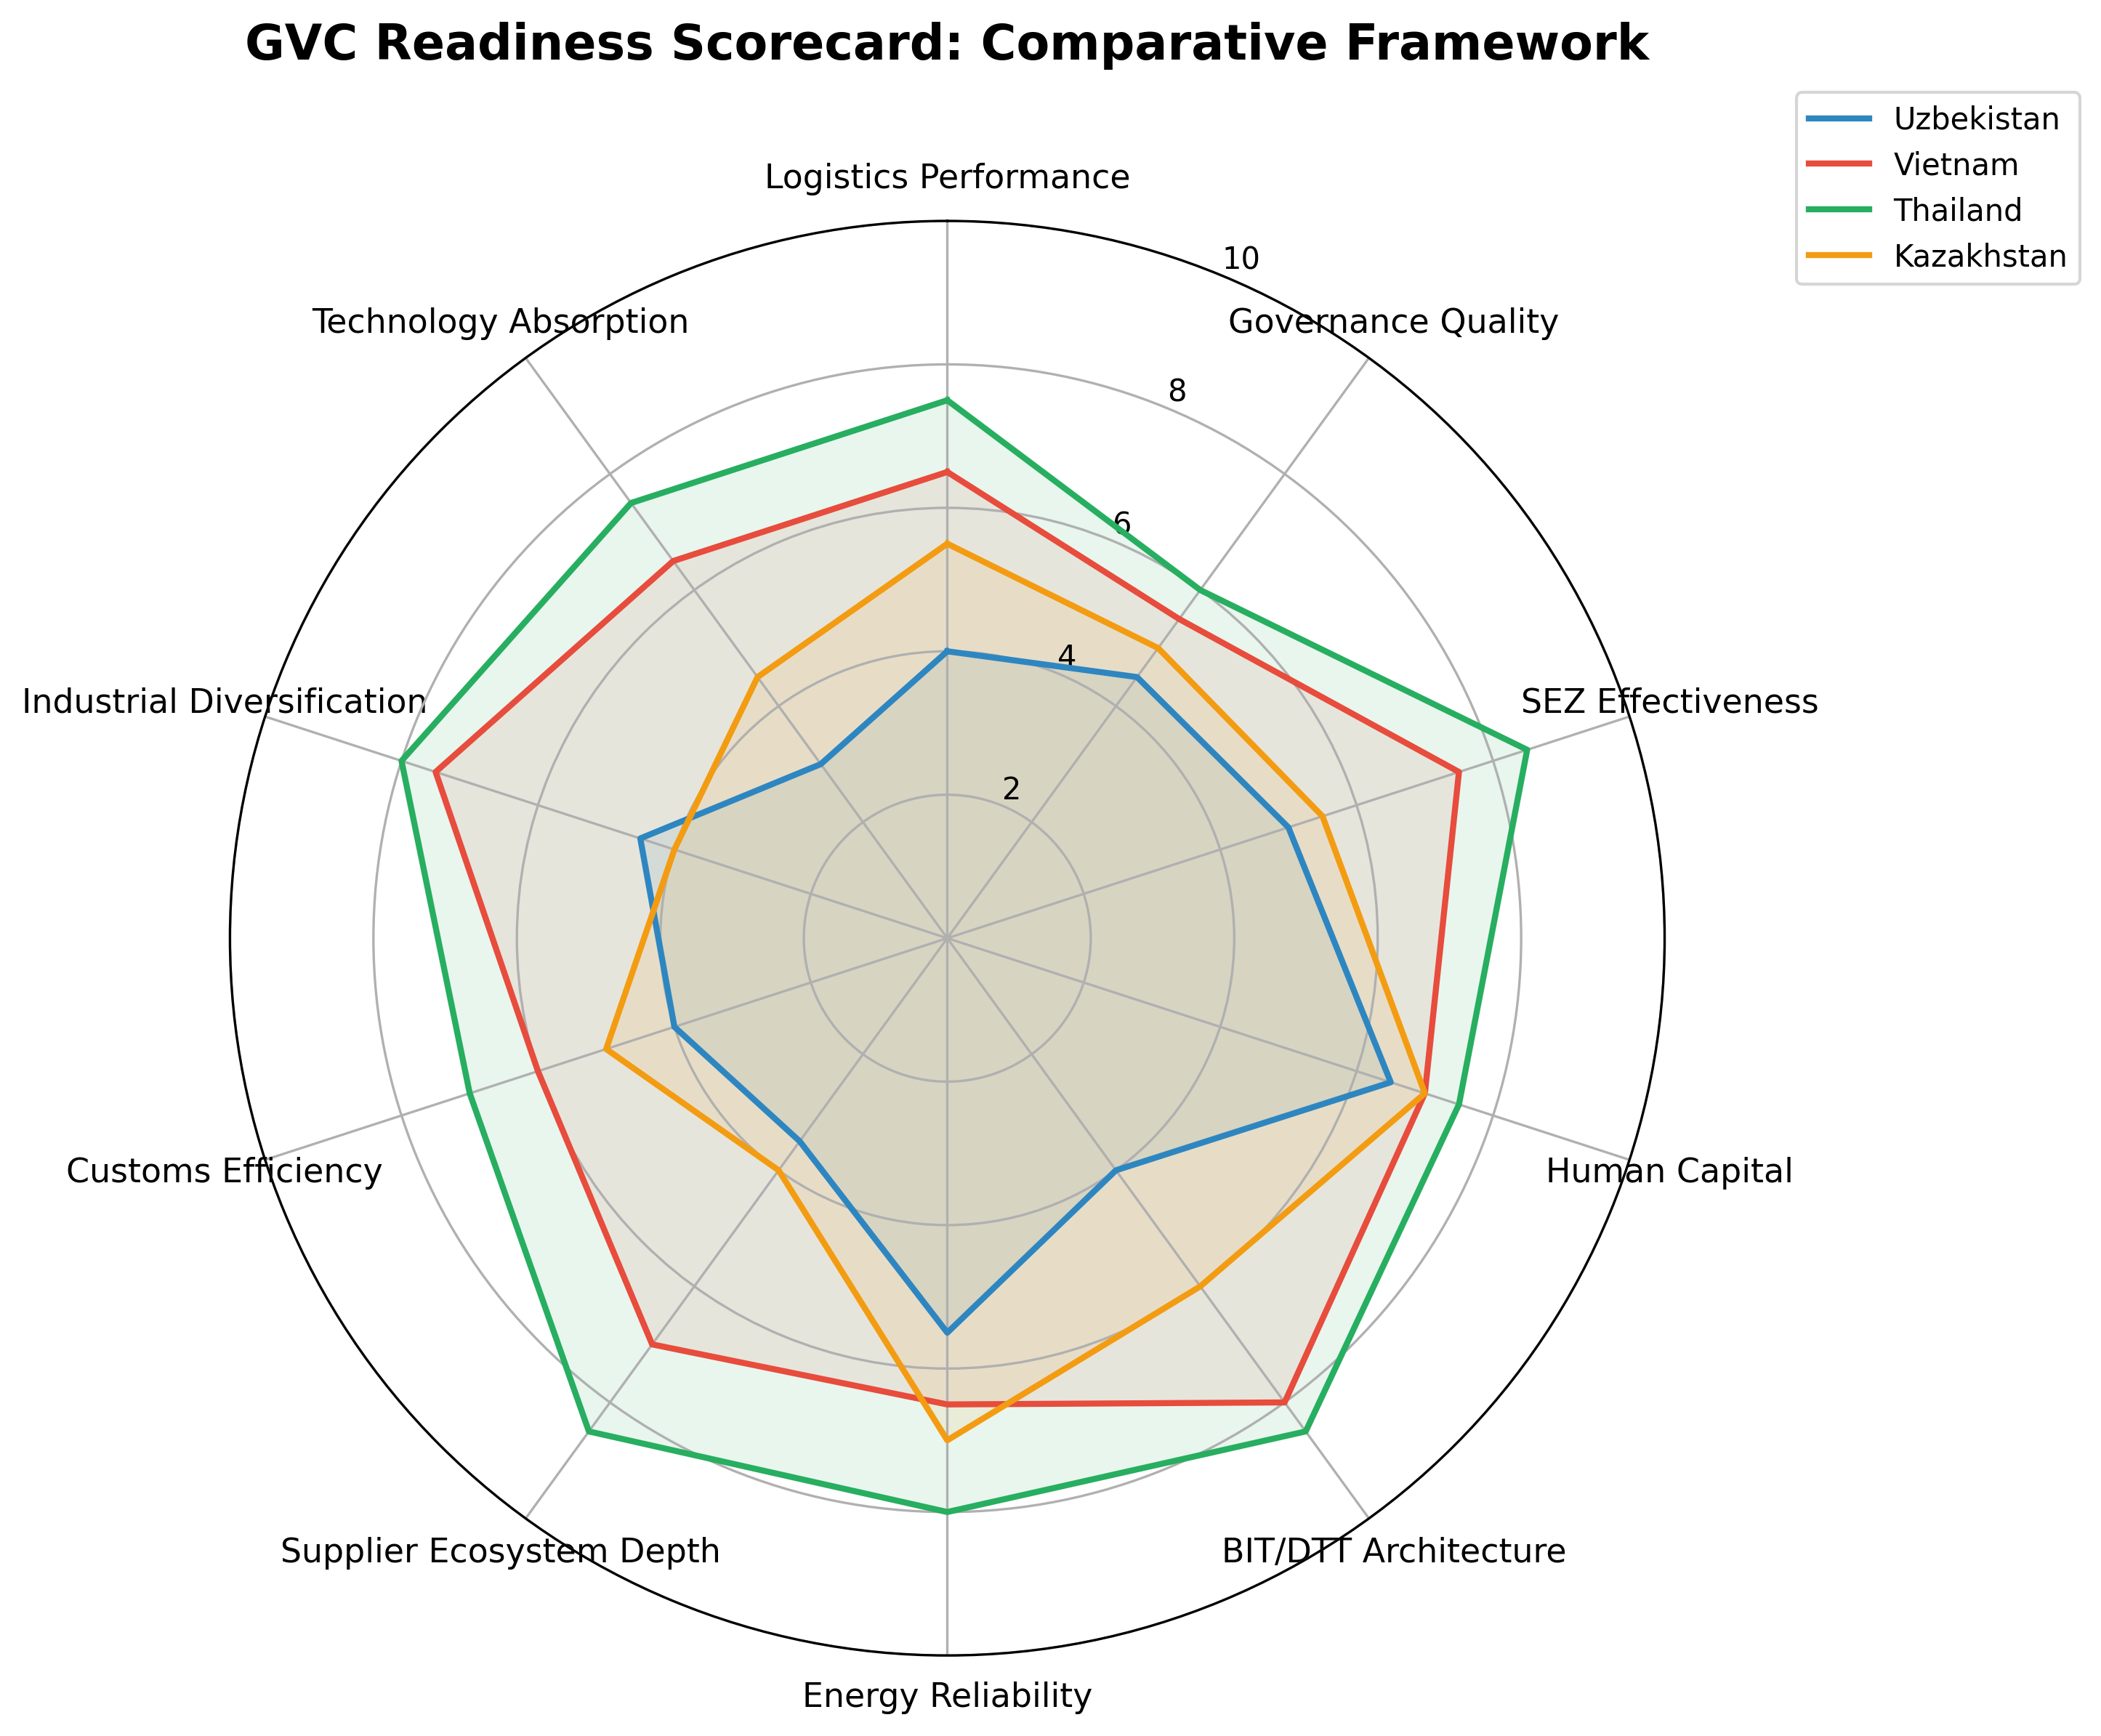
\includegraphics[width=0.85\textwidth]{figures/gvc_readiness_radar.png}
    \caption{Comparative GVC Readiness: Uzbekistan vs. Benchmark Economies}
\end{figure}

\subsection{Scorecard Results \& Gap Analysis}

\begin{table}[h!]
\centering
\rowcolors{2}{gray!10}{white}
\begin{tabularx}{\textwidth}{l C C C C}
\toprule
\rowcolor{adbblue}\textcolor{white}{\textbf{Indicator}} & \textcolor{white}{\textbf{Uzbekistan}} & \textcolor{white}{\textbf{Vietnam}} & \textcolor{white}{\textbf{Thailand}} & \textcolor{white}{\textbf{Kazakhstan}} \\
\midrule
Logistics Performance & 4.0 & 6.5 & 7.5 & 5.5 \\
Governance Quality & 4.5 & 5.5 & 6.0 & 5.0 \\
SEZ Effectiveness & 5.0 & 7.5 & 8.5 & 5.5 \\
Human Capital & 6.5 & 7.0 & 7.5 & 7.0 \\
BIT/DTT Architecture & 4.0 & 8.0 & 8.5 & 6.0 \\
Energy Reliability & 5.5 & 6.5 & 8.0 & 7.0 \\
Supplier Ecosystem Depth & 3.5 & 7.0 & 8.5 & 4.0 \\
Customs Efficiency & 4.0 & 6.0 & 7.0 & 5.0 \\
Industrial Diversification & 4.5 & 7.5 & 8.0 & 4.0 \\
Technology Absorption & 3.0 & 6.5 & 7.5 & 4.5 \\
\midrule
\textbf{Composite Score} & \textbf{4.45} & \textbf{6.80} & \textbf{7.70} & \textbf{5.35} \\
\bottomrule
\end{tabularx}
\caption{GVC Readiness Scorecard Matrix}
\end{table}

\textbf{Strategic Imperative:} Uzbekistan’s primary binding constraints are Logistics (4.0) and Technology Absorption (3.0). To move from "Captive" to "Relational" governance, policy must pivot from generic investment attraction to targeted supplier upgrading and transport corridor acceleration.

\newpage
% ---------------------------------------------------------
\section{OUTPUT 2: Sector Targeting Matrix}
% ---------------------------------------------------------

\subsection{Strategic Rationale}
Traditional IPAs often target sectors based on generic domestic endowments. This matrix redirects targeting toward sectors that fit landlocked constraints and align with Northeast Asian supply chain restructuring (China+1 strategies).

The matrix evaluates sectors on four dimensions:
\begin{enumerate}
    \item \textbf{Value-to-Weight Ratio:} High priority for landlocked states to overcome transit costs.
    \item \textbf{Technology Spillover Potential:} Capacity to generate tacit knowledge transfer.
    \item \textbf{NE Asian Investor Interest:} Alignment with Japanese, Korean, and Chinese out-migration trends.
    \item \textbf{Local Compatibility:} Match with existing Uzbek infrastructure and labour skills.
\end{enumerate}

\subsection{Prioritisation Matrix Dashboard}

\begin{figure}[h!]
    \centering
    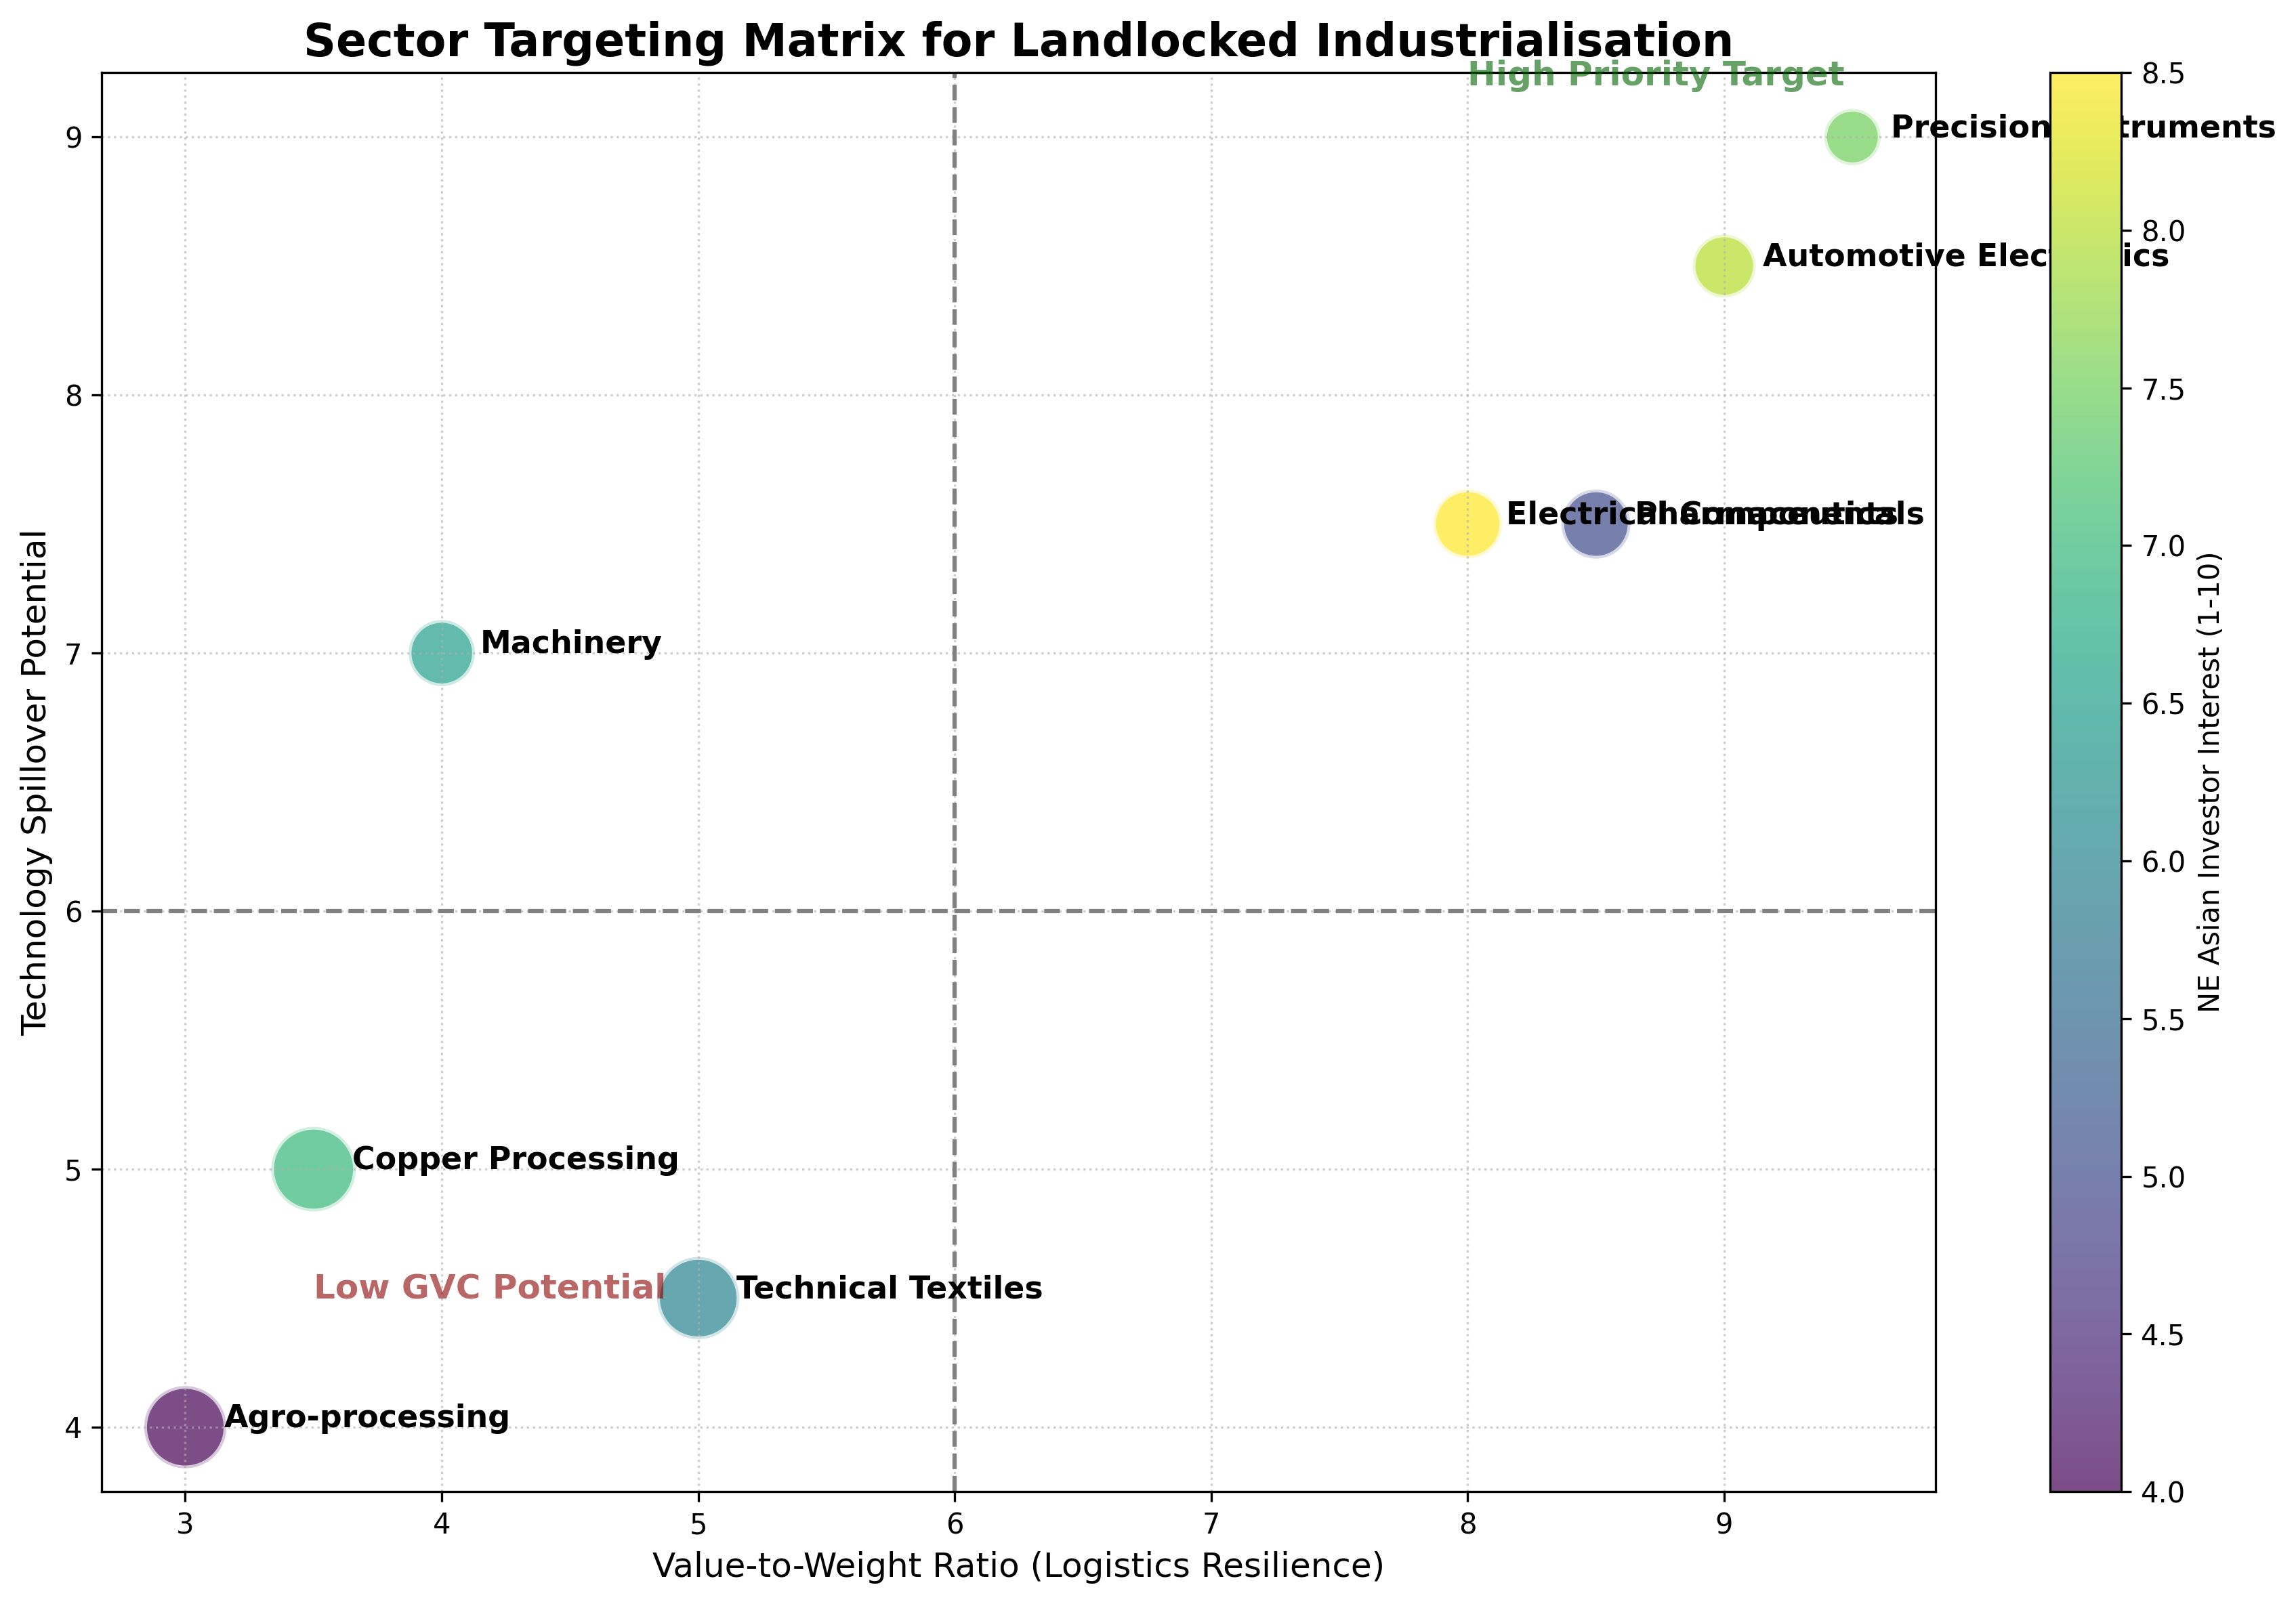
\includegraphics[width=0.85\textwidth]{figures/sector_targeting_matrix.png}
    \caption{Sector Prioritisation: Value-to-Weight vs. Tech Spillover}
\end{figure}

\subsection{Targeting Recommendations}

\begin{itemize}
    \item \textbf{Tier 1 (Immediate High Priority):} \textit{Automotive Electronics, Electrical Components}. High value-to-weight ratio minimizes logistics penalties. Aligns perfectly with Korean (e.g., Samsung SDI, Hyundai) and Chinese EV supply chain relocation.
    \item \textbf{Tier 2 (Medium Term / Niche):} \textit{Pharmaceuticals, Precision Instruments}. Requires specific SEZ environments (clean rooms, cold-chain logistics, Navoiy cargo integration).
    \item \textbf{Tier 3 (Current Cash Cows but Low GVC Potential):} \textit{Technical Textiles, Copper Processing}. High local compatibility but low technology spillover and highly vulnerable to rail/road logistics costs. Move downstream to higher value-add.
\end{itemize}

\newpage
% ---------------------------------------------------------
\section{OUTPUT 3: Policy Trigger Framework}
% ---------------------------------------------------------

\subsection{Overview}
Static economic scenarios fail to provide actionable feedback loops for policymakers. This framework converts the dissertation’s trajectory analysis into a dynamic, monitorable trigger system. When specific threshold triggers are met, institutional responses are automatically mandated.

\textbf{Empirical Foundation:} The empirical findings of this dissertation---specifically the non-significant FDI coefficient alongside the significant intermediate goods share coefficient ($\beta = 2.34$, $p < 0.05$)---suggest that the mechanism for manufacturing upgrading operates through production network embedding rather than through investment volume alone. This implies that policies targeting FDI quantity (tax holidays, land cost subsidies) are second-order instruments; first-order instruments are those that deepen intermediate goods trade relationships (supplier development programmes, backward linkage requirements). The triggers below operationalise this finding.

\subsection{Implementation \& Response Matrix}

\renewcommand{\arraystretch}{1.4}
\begin{longtable}{p{4cm} p{3cm} p{4.5cm} p{3.5cm}}
\toprule
\rowcolor{adbblue}\textcolor{white}{\textbf{Trigger Condition}} & \textcolor{white}{\textbf{Threshold Target}} & \textcolor{white}{\textbf{Policy Response / Action}} & \textcolor{white}{\textbf{Lead Institution}} \\
\midrule
\endhead

\textbf{1. Logistics \& Transit} \newline Customs clearance time for intermediate goods & $< 24$ hours sustained for 1 quarter & Elevate SEZ status to "Green Channel" for Top 50 exporters; implement automated pre-clearance. & State Customs Committee \\
\midrule
\textbf{2. FDI Composition} \newline Japanese/Korean FDI as \% of Total Inflows & $> 10\%$ annual share & Activate "Tier 1" Supplier Upgrading Fund to co-finance domestic SMEs supplying these anchor firms. & Ministry of Investment / IPA \\
\midrule
\textbf{3. Infrastructure} \newline CKU (China-Kyrgyzstan-Uzbekistan) Railway & Operational / Cargo Phase 1 & Re-zone Fergana Valley industrial parks specifically for time-sensitive component assembly. & Ministry of Transport / MIFT \\
\midrule
\textbf{4. Domestic Linkages} \newline Local content in targeted manufacturing sectors & $< 15\%$ after 3 years of operation & Implement mandatory technology transfer audits; review SEZ tax exemption renewals based on linkage targets. & Ministry of Economy \\
\midrule
\textbf{5. Export Sophistication} \newline Share of HS-84/85 (Machinery/Electronics) & $> 12\%$ of non-gold exports & Transition from generalized SEZs to specialized Tech-Parks with dedicated R\&D infrastructure. & Agency for Innovative Development \\

\bottomrule
\end{longtable}

\textbf{Risk-Response Protocol:} If Trigger 4 (Local Content) remains below threshold, it indicates a "Captive Governance Trap." The immediate policy response is to cease generic tax holidays and pivot entirely to co-financing worker training and SME technological upgrading.

\newpage
% ---------------------------------------------------------
\section{OUTPUT 4: Firm-Level Survey Instrument}
% ---------------------------------------------------------

\subsection{Objective and Methodology}
This survey is designed for administration to foreign manufacturing firms operating in Uzbekistan's Special Economic Zones. The objective is to empirically determine the GVC governance structure (Captive vs. Modular vs. Relational) and quantify the depth of technology transfer. 

\textbf{Implementation Guide:} Administer annually via the IPA. Responses should be Likert-scale (1-5) or categorical. Data must be anonymized to ensure accurate managerial reporting.

\subsection{Survey Questionnaire}

\textbf{Module A: Supplier Linkages \& Sourcing}
\begin{enumerate}
    \item What percentage of your intermediate material inputs (by value) are sourced from domestic Uzbek suppliers? \textit{( $<5\%, 5-15\%, 16-30\%, >30\%$ )}
    \item How would you rate the technical capacity of your domestic suppliers to meet global quality standards? \textit{(1=Severely Lacking, 5=World-Class)}
    \item Does your firm actively provide technical blueprints, financing, or engineering support to local suppliers? \textit{(Yes / No / Planned)}
\end{enumerate}

\textbf{Module B: Autonomy and Governance Structure}
\begin{enumerate}
  \setcounter{enumi}{3}
    \item Where are core product design and R\&D decisions made? \textit{(Headquarters abroad / Regional Hub / Local Uzbek Subsidiary)}
    \item Can the Uzbek subsidiary independently modify production processes or source new suppliers without HQ approval? \textit{(1=No Autonomy, 5=Complete Autonomy)}
    \item Are your exports from Uzbekistan primarily intra-firm (shipped to your own facilities in other countries) or to independent buyers? \textit{(Primarily Intra-firm / Mixed / Independent)}
\end{enumerate}

\textbf{Module C: Workforce and Technology Transfer}
\begin{enumerate}
  \setcounter{enumi}{6}
    \item What percentage of management and senior engineering roles in your Uzbekistan facility are held by local citizens? \textit{( $<10\%, 10-30\%, 31-50\%, >50\%$ )}
    \item How many weeks of formal technical training does the average production worker receive annually?
    \item Does your facility employ proprietary manufacturing technologies that are unique to your firm within Central Asia? \textit{(Yes / No)}
\end{enumerate}

\textbf{Analytical Key:}
\begin{itemize}
    \item \textbf{Captive Governance Profile:} High intra-firm trade (Q6), low local sourcing (Q1), low subsidiary autonomy (Q4, Q5), minimal local management (Q7).
    \item \textbf{Relational Governance Profile:} Increasing local sourcing (Q1) coupled with active supplier support (Q3), mixed/independent exports (Q6), and higher autonomy/local management (Q5, Q7).
\end{itemize}

\newpage
% ---------------------------------------------------------
\section{OUTPUT 5: Policy Brief}
% ---------------------------------------------------------

\begin{center}
    {\Large\color{adbblue}\textbf{The Navoiy Model: Air-Cargo Logistics as a Strategy for Landlocked Industrialisation}}\\[1em]
    \textit{Policy Briefing Note}
\end{center}
\vspace{1em}

\subsubsection*{1. Executive Summary}
For landlocked developing countries (LLDCs), traditional export-led industrialisation is fundamentally constrained by the "distance penalty"—the time and cost of overland transit to maritime ports. Uzbekistan’s Navoiy Free Industrial Economic Zone (FIEZ), anchored by a dedicated air-cargo hub managed in partnership with Korean Air, represents a paradigm shift. This brief argues that air-cargo industrialisation is the most viable strategy for integrating LLDCs into Northeast Asian electronics and pharmaceutical value chains.

\subsubsection*{2. The Landlocked Development Problem}
Uzbekistan faces a double-landlocked geography. Traditional manufacturing models relying on containerized ocean freight (the "Vietnam/Thailand model") are structurally incompatible with the logistics realities of Central Asia. The transit time to major ports exceeds the inventory-holding tolerance of modern just-in-time (JIT) electronics manufacturing, effectively locking the country out of high-tech Global Value Chains (GVCs).

\subsubsection*{3. Navoiy as an Alternative Logistics Model}
The Navoiy model bypasses terrestrial bottlenecks by linking manufacturing directly to an international air corridor. By creating a customs-free zone physically adjacent to an air-freight terminal, components manufactured in Incheon or Shenzhen can arrive in Navoiy, undergo final assembly, and be airlifted to European markets within 48 hours. This neutralizes the geographic penalty.

\subsubsection*{4. Product Categories Suitable for Air-Freight}
Air-freight industrialisation is not sector-agnostic. It requires products with an exceptionally high value-to-weight ratio and high time-sensitivity. Target sectors include:
\begin{itemize}
    \item \textbf{Automotive Electronics \& Sensors:} Lightweight, high-value components.
    \item \textbf{Active Pharmaceutical Ingredients (APIs) \& Biologics:} Requiring strict cold-chain and rapid transit.
    \item \textbf{Precision Instruments \& Medical Devices.}
\end{itemize}
Heavy manufacturing, such as white goods or basic textiles, cannot absorb air freight premiums and remains reliant on rail corridors.

\subsubsection*{5. Replicability and Policy Recommendations}
To scale the Navoiy model, policymakers must treat aviation infrastructure as industrial policy infrastructure. 
\begin{itemize}
    \item \textbf{Align SEZ Incentives with Air-Freighted Sectors:} Cease allocating prime land in air-linked SEZs to low-value, heavy-industry firms. Restrict entry strictly to high value-to-weight manufacturers.
    \item \textbf{Integrate Customs Architectures:} Implement "pre-arrival processing" so that air-cargo components clear customs while mid-flight, achieving true JIT capability.
    \item \textbf{Expand "Fifth Freedom" Traffic Rights:} Liberalize airspace policies to allow foreign cargo carriers to utilize Navoiy as a regional distribution hub without restrictive bilateral quotas.
\end{itemize}

\subsubsection*{6. Conclusion}
The Navoiy air-cargo industrialisation model proves that geography is not destiny. For Uzbekistan to capture Northeast Asian GVC relocation, it must aggressively market its air-logistics capabilities to Korean and Japanese firms, treating the airport not merely as transport infrastructure, but as the primary conduit for industrial upgrading.

\end{document}
